\chapter{A bit  of logic, some more parts of the interface, and writing more compact and idiomatic proofs}

\section{Why logic?}
Now that you've used Isabelle for a while, you've seen the difference between the kinds of things you can write when you're telling Isabelle \textit{what} to do (e.g., ``show \textit{this} using \textit{that} by \textit{that method})'' and telling it what to do it \textit{to} (i.e., the ``this'' of the previous sentence).  

The first of these is called \term{outer syntax}, and the second \term{inner syntax}. In our use-case, the inner syntax describes `HOL' a higher-order logic that I'll do my best to describe informally but without too many lies. The distinction between inner and outer is less clear than the names might suggest, because Isabelle allows a logic like HOL to introduce new syntax at the outer syntax level. As an example, in HOL you can define a new datatype. In Isabelle/HOL, you can do this with code like this:
\begin{IS}
datatype f = Zero | One | Two
\end{IS}
which looks like outer syntax, and indeed is \ldots because HOL defined it. 

We need an understanding of the logic HOL, but more importantly, of what a logic \textit{is}) to use Isabelle sensibly. The next section attempts to provide this. 
\section{
A Very Incomplete and Informal Introduction to Some Logic, Deduction, and its relationship to Isabelle}

Most mathematicians know some logic, and say with varying degrees of confidence that if $A$ implies $B$ then $(\neg B)$ implies $(\neg A)$, and similar things. Constructivists don't like that sort of thing, but it's very much a part of Isabelle/HOL, which is what I'm writing about, so I'm just going to ignore their concerns. 

What are $A$ and $B$ here? In the simplest logic (``Propositional logic'') they're symbolic representations of statements about the world, so $B$ might stand for ``My dog is a poodle'' and $A$ might stand for ``the sun is shining''. We think of them standing for assertions that are either true or false (called propositions). In this case, B is actually false, while A is true, but if I'd said that B and A represented different statements, B might have been true and A false. In this example, B and A are called ``atomic'' because they cannot be broken into simpler things, while something like ``I like coffee and I like tea'' can be broken into a conjunction of C (I like coffee) and D (I like tea). So we have both atomic and compound propositions. 

The rule for forming compound propositions is that we can use various ``connectives'' like ``and'' ($\wedge$), ``or'' ($\vee$) and ``not'' ($\neg$) (which for now we should regard as mere symbols with highly-suggestive names), and also ``implies'' ($\to$). This lets us take some atomic propositions like A, B, C and form from them more complex propositions like $A \wedge C$ or $B\vee (\neg D) \to B$. These compound propositions may be true or false --- that's a separate matter from whether they are in fact propositions. So this paragraph discusses only how we may \textit{form} propositions, and nothing about their truth or falsehood. Everything here may be regarded as essentially textual: we can take a proposition A and another B and put the symbol `$\wedge$' between them and we have a new proposition. B might be atomic or complex --- it doesn't matter. It's also worth noting some things that are \textit{not} ways to form propositions: you can't just place two propositions next to each other like this: $AB$. You can't put two binary connectives next to each other, like $A \to \wedge B$. The connective $\neg$ is unary, so you \textit{can} form $A \wedge \neg B$, which is to be parsed as $A \wedge (\neg B)$.

It's probably best to regard (for the time being) all such combinations as including parentheses, as in $(A) \wedge (B)$, so that if we combine $P \to Q$ with $R  \wedge S$, we get $(P \to Q) \wedge (R  \wedge S)$ rather than $P \to Q  \wedge R \wedge S$, which might be read as $(P  \to (Q  \wedge R)) \wedge S$, a proposition that could be formed using a quite different sequence of combinations.  

Our understanding of truth-values (the ``True'' and ``False'' of Boolean logic) and of the intuitive meaning of the connectives let us assign a truth value to a compound proposition once we have truth values for its atomic constituents. Such an assignment of truth values (first to atomic propositions, and then by rules of logic to every proposition) is called an ``interpretation'' by logicians. 

A proposition like $A \to A$ is interesting in part because no matter what value (T or F) we assign to $A$, the (compound) proposition $A \to A$ is always true. Such a proposition is called a \term{tautology}.

You might reasonably think that such a proposition would be easy to prove! But a modern 'logic' not only assigns a truth value to each proposition for a given interpretation, it also includes \term{rules of deduction} --- ways to get from one or more propositions to another, and those rules of deduction govern what can be ``proved''. 
(Thus ``provable'' and ``has to be true in every interpretation'' are different notions, which takes a little getting used to!)  You can think of these 'deductive rules' almost as textual-pattern-matching-and-replacement rules. At any step of a deductive process, we have some number of 'facts' (propositions known to be true for some reason) --- also called a \textit{context} --- and we can use a deductive rule to generate new facts. 

As an instance of this, a fairly standard deductive rule is that if we have, in our current context (i.e., collection of known facts), the facts $P$ and $Q$, then we can deduce $P\wedge Q$. But you can imagine an impoverished logic that has no deduction rules at all. In such a logic, knowing $P$ and $Q$ doesn't let you deduce $P \wedge Q$. 

Another rule (again, constructivists will balk) is that for any proposition P, we can deduce (from nothing!) the proposition $P\vee(\neg P)$. That's a useful deduction rule to have, as it provides a way to get started in assembling a bag of facts that we carry with us in creating a proof.

If a set of deductive rules is rich enough to allow it to prove all tautologies, it's said to be \term{complete}. Completeness is absolutely desirable, but there are perils: imagine a deductive scheme in which we have a rule that ``no premises at all'' allows us to conclude any proposition $X$ whatsoever. In such a scheme, we can deduce any formula, hence we can deduce any tautology, so it \textit{is} complete. But it also allows us to deduce many false formulas, so it's hardly one we'd want to use. The dual idea is \term{soundness}: a set of deduction rules is \term{sound} if all the things we can deduce are tautologies. Once again, soundness isn't everything: a deductive scheme with no rules at all is sound, because it doesn't allow us to deduce anything at all! But a sound-and-complete set of deductive rules is the sweet spot: it gives us the confidence that we can only prove the kinds of things we want to prove, but also that any such thing can be proven. If you had to give up one of the two properties in selecting a deductive scheme for a proof-assistant, you'd probably regretfully choose to abandon completeness. You'd say ``We can't help you prove everything, but at least the things we help you prove will all be true, and while we might miss some things, we're able to prove a ton of stuff, so that's good.'' 

As it happens, for propositional logic, there's a set of deduction rules that is both sound and complete. That's great news. Unfortunately, for first-order logic (which allows ``for all'' and ``there exists'') there's no such set of deduction rules. And for higher-order-logic (HOL), which we'll soon discuss, things are even worse. Logic courses delight in showing these things, but I'm going to stop after one more paragraph and discuss them no further. 

I've talked about proving tautologies, but what if something is \textit{not} a tautology? Can we prove that it's not? More explicitly, suppose we have an interpretation in which some formula is false. Would a sound-and-complete deduction scheme help us know that? Not necessarily. So even sound-and-completeness isn't a be-all and end-all. 

There's a set of deduction rules (one that matches very well with my own sense of what's reasonable!) with the somewhat loaded name \term{natural deduction}. These are rules not for propositional logic, but for \term{first-order logic}, which is a logic that includes the notions ``for all'' and ``there exists''. Within first-order logic, we also have a notion of predicates, which look like functions of one or more arguments whose value may be true or false. For instance, with the assignment of truth values to $A$ and $B$ from a few paragraphs back ($B$ was false, $A$ was true),  the predicate $P(x) = x$ is true for $x = A$, but false for $x = B$. One of the rules of natural deduction is that if you know $\forall  x . P(x)$, then you know $P(a)$. Another is that if you know $P(a)$, then you know $\exists x . P(x)$. In our case, we know $P(A)$, so we can deduce that $\exists x . P(x)$. 

Let me now walk you through some of the basic rules of natural deduction, because they have some fairly standard names that come up in Isabelle, and if (like me) you don't know them, you find yourself saying ``What the heck is 'allE'?'' None of them are particularly surprising, so this will just be an exercise in naming. It's helpful, in describing these things, to use a notation developed by Gentzen, in which there's a horizontal line that indicates deduction. Things above the line, separated by commas, indicate a portion of the currently-known context; things below indicate something you can deduce from such knowledge. For instance, the rule that if you know that $P$ implies $Q$ and you know $P$, then you know $Q$ (a rule that is called \term{modus ponens}), gets written like this:

\begin{verbatim}
    
P -> Q, P
-------------
      Q
\end{verbatim}


It should come as no surprise that there are other notations as well, but I'll stick with this one. I like to think of the comma above the line as denoting the words ``as well as'', so that this says `if you know $P \to Q $ as well as $P$, then you can conclude $Q$.' Using "as well as" avoids the informal use of "and", which is easy to confuse with the $\wedge$ symbol.

Let's start with a very simple one: ``and-introduction''. It says that if you know $P$ as well as $Q$, then you can deduce $P \wedge  Q$. The shorthand name for this is conjI (Here ``conj'' is short for ``conjunction'', a fancy way to say ``and''; the corresponding thing for ``or'' is ``disjunction''. The ``I'' at the end is for ``introduction'', because this introduces a new conjunction to our set of known facts). And the pictorial representation is

\begin{prooftree}
\AxiomC{$P, Q$}
\LeftLabel{ConjI:}
\UnaryInfC{$P \wedge Q$}
\end{prooftree}

I've written ``conjI'' next to the horizontal line because in a long sequence of deductions, it can be nice to have a ``reason'' for each statement in a proof, and just to the left of the line seemed like a good place to put it. 

Brief digression to relate this to our bigger picture, namely proofs in Isabelle. Suppose you've managed to show some fact $B$ and some other fact $D$. (Maybe $x$ is some real number, and $B$ says $x < 7$ while $D$ says $x > 3$.) If Isabelle has these two facts, it can deduce the fact $B \wedge D$ or the fact $D \wedge B$ using ``conjI'' (i.e., in either case concluding that $3 < x$ and $x < 7$.) If we were focusing on something called \term{apply-style} proofs, we might actually mention the name ``conjI'' in some proof. (We're not, so that's the last I'll say about it for some time.)

The ``I'' in conjI refers to ``introduction'' because once we apply this rule, there's a new ``$\wedge$'' in our bag of facts. Several of the natural-deduction rules are ``introduction rules'', and for each, there's a corresponding ``elimination rule''.

Within Isabelle, there are lots of introduction- and elimination-rules, and they get used by various provers, and a good proof-writer will be sure to add new rules following definitions of new things. For instance, we might have added an elimination rule for the subtraction operation, saying that we can always change \isi{x - y} into \isi{x + (neg y)}, thus eliminating the subtraction operation. Presently we'll return to those Spivak proofs and do just this, and see how much simpler they become. 

Along with and-introduction come two closely related rules, one that says that if you know $P \wedge  Q$, then you know $P$, and the other that says that if you know $P \wedge  Q$, then you know $Q$,
\begin{prooftree}
\AxiomC{$P \wedge Q$}
\LeftLabel{ConjE1:}
\UnaryInfC{P}
\end{prooftree}

\begin{prooftree}
\AxiomC{$P \wedge Q$}
\LeftLabel{ConjE2:}
\UnaryInfC{Q}
\end{prooftree}

The ``E'' here is for ``elimination'', which has always seemed like a misnomer to me: if you know $P \wedge  Q$ before applying this rule, you also know it after doing so; you just happen to also know $P$. But ``introduce'' and ``eliminate'' are verbal opposites, so perhaps it's not a bad name. And you can, after all, go from knowing $P \wedge Q$ to knowing $P \wedge Q$ and $Q$ (using conjE2) and then choose to forget about $P  \wedge  Q$ if you're not going to need it again. 

The situation for ``or'' is almost exactly dual: there are two or-introduction rules, but only one or-elimination rule. But the elimination rule takes a somewhat surprising form. First, the introduction rules:

\begin{prooftree}
\AxiomC{$P$ }
\LeftLabel{DisjI1:}
\UnaryInfC{$P \vee Q$}
\end{prooftree}

\begin{prooftree}
\AxiomC{$Q$ }
\LeftLabel{DisjI2:}
\UnaryInfC{$P \vee Q$}
\end{prooftree}

You might be asking why you'd ever want to use or-introduction. Well, imagine if your Isabelle goal has a  $ \vee $ in it --- it's something like \isi{ n = 0   \<vee>  n*n > 0}. You know that in the current sub-proof, $n$ actually \textit{is} zero, and you feel that you should be able to claim that you've proved the goal. But ``\isi{ n = 0 }'' and ``\isi{ n = 0   \<vee>  n*n > 0}'' are textually distinct and to get that ``$\vee$ '' into the collection of facts, you're going to need or-introduction. There's good news, though: you seldom need to use it explicitly, because there are a couple of proof-methods in Isabelle (``fastforce'', ``force'', and ``blast'') that can do a lot of things in this simple realm and beyond. But sometimes you really need one of these rules to nudge Isabelle in the right direction, and it helps to know they exist and what their names are. 

The or-elimination rule takes, as its context, both a disjunction, $P \vee Q$, and two \textit{derivations}, i.e., sequences of legal deductions, one leading from $P$ to $R$ and another leading from $Q$ to $R$. These, taken together, let you conclude $R$. Note that the deduction from $P$ to $R$ doesn't say that $P$ is true! Instead, it says that \textit{if} $P$ is true, you can deduce that $R$ is true. The same goes for the deduction from $Q$ to $R$: it asserts nothing about the truth of $Q$, only about what's provable if $Q$ is true. In Isabelle/HOL (which you can see in \$ISABELL\_HOME/src/HOL), the long right arrow is used to mean ``is derivable from'', so the statement of the disjunction-elimination rule is this:


We'll ignore the proof here, and simply see that it says what was discussed about: if we know $P \vee Q$, and know $R$ is derivable from $P$ and also derivable from $Q$, then we can conclude $R$. 

If you think for a moment, this makes a lot of sense as an elimination rule: from ``P or Q'' you can't conclude either P or Q, but you know at least ONE of them has to be true, so if you can derive something interesting from each one, then that derived thing must be true. For instance, if you know $t$ is one of the two numbers $3$ or $7$, and $f(x) = (x-5)^2 - 4$, then you can conclude that $f(t) = 0$ without knowing which of the two values $t$ actually has!

Side note: with this in mind, and what you've already seen of Isabelle, you may now find the early parts of ``Programming and Proving'' somewhat more readable.

Indeed, you may be ready to start seeing how Isabelle is doing some of its magic by looking through \$ISABELLE\_HOME/src/HOL, starting at the subsubsection called ``Axioms and basic definitions'', as long as you don't try to really understand everything. For instance, the 'axiom' that from knowing that $s = t$, you can derive $P s = P t$ \ldots  that seems pretty reasonable. That's just the substitution we're used to doing all over mathematics (and indeed, that rule is called ``subst''). Some of the other things that follow are, like \isi{disjE}, harder to grasp unless you think for a while. 

Isabelle/HOL is a little bit baffling to beginners because there are two different logics. There's the ``outer syntax'' logic which can do a lot of things that the inner syntax cannot, but which really knows almost nothing about any kind of mathematics -- things like $3 < 11$ and the Intermediate Value Theorem are, to it, mere black boxes. Where it excels is in gluing together these black boxes into a chain of reasoning. So if it knows the facts that (1) $f$ is a real-to-real function, (2) $f$ is continuous, (3) $f(0) = 6$, (4) $f(1) = -5$, and the intermediate value theorem, it can conclude that there's a number $c$ between $0$ and $1$ with $f(c) = 0$. [To be honest, it also needs to know that $6 > 0$ and that $-5 < 0$, because those come up in the hypotheses of the IVT as well.] 

There is also ``glue'' between the outer and inner syntax. Implication in HOL is written ===>, and there's a rule (impI) that says this:

I.e., if we want to show that P implies Q, it's sufficient to show that using the outer logic

Recommended reading: Consider reading through a good chunk of the Wikipedia article on natural deduction (https://en.wikipedia.org/wiki/Natural\_deduction as of 4/28/2023) to get a somewhat more authoritative and thorough description of it. 

Arrows and 'and' and implications and bags of facts
If you have a choice between (a) knowing P, Q, and that having both allows you to conclude R and (b) knowing ``$P  \wedge  Q \implies R$'', in Isabelle you should definitely prefer the first, because most of the provers are better at working with the first than the second. We've used fix-assume-show form for this kind of thing. If we have a theorem of the form

\begin{IS}
theorem:
   assumes P and Q   
   shows R
proof <details here\ldots > qed
\end{IS}


this can also be written as 
\begin{IS}
theorem:
   [[P; Q]] ===> R
\end{IS}

where the double-brackets indicate a list of things we need to know in order to conclude R using this theorem, i.e., they tell us what needs to be in our current context. Our context might contain P and Q in either order, or widely separated in its list of facts, and that's OK. This is, of course, much less rigid than knowing that ``$P  \wedge  Q -> R$'', because to apply that theorem, we need to have established ``$P  \wedge  Q$'' (and not ``$Q  \wedge  P$''!). Even if $P$ and $Q$ are in our context, that requires an initial and-introduction step. 

That double-bracket form is often replaced, much to my consternation when I was starting out, with this: 

\begin{IS}
    P ===> Q ===> R

\end{IS}
which doesn't seem at all the same. Once you realize that the arrows associate to the right, this says \isi{P ===> (Q ===> R)}, or in English, ``Knowing $P$ lets you conclude that if you know $Q$, then you know $R$'', or, in simpler terms, ``knowing both $P$ and $Q$ lets you conclude $R$.'' In much the same way, it could be replaced with ``\isi{Q ===> (P === R)}'', which is also equivalent. 

To do: the problem when you want to unify P with this second form. Solution: you can rotate the assumptions (see zulip)

In much the same way, in propositional logic, $(p -> q) -> r$ is the same as $(p  \wedge  q) -> r$.

There's one more aspect to HOL that we've used but that I haven't mentioned: there's a notion of types, like int, or nat, or bool, and ways to construct new types from old (as in ``int set'' or ``int => nat''), and everything in HOL has a type. In ordinary propositional logic, if you want to claim that for natural numbers, n < 2n+1, you have to say ``for all $n$,  $n$ is a natural number implies that  $n < 2n + 1$.'' In HOL, you say ``for all naturalnumbers $n$, $n < 2n + 1$''. That saves a lot of grief in trying to express things, which you'll grow to appreciate. 

To do: ConjI and ConjE and AllI using \ldots however you search! \ldots  and give details here. Also AllI, AllE, SomeI, SomeE

By the way, doing logic proofs using basic inference rules can be a pain, but there are tools to help you. Consider this problem from math.stackexchange.com, slightly edited:


\begin{quote}   
We have these two assumptions: (a) “Logic is difficult or not many students like logic.” and (b) “If mathematics is easy, then logic is not difficult.”

By translating these assumptions into statements involving propositional variables and logical connectives, can we determine weather the following statement is valid conclusion of these assumptions using rules of inference?

\emph{If not many students like logic, then either mathematics is not easy or logic is not difficult.}

[...]

I have used these logical variables
$l$: logic is difficult; $s$: many students like logic; 
$m$: mathematics is easy.

By translating we have:
\begin{align}
l \vee \neg s \\
m \to \neg l
\end{align}
and we want to conclude 
\begin{align}
\neg s \to (\neg m \vee \neg l)
\end{align}
\end{quote}
We can actually use an online resource \href{https://www.umsu.de/trees/#(q~1(~3s))~1(m~5(~3q))~5((~3s)~5((~3m)~2(~3q)))}{online resource} to answer this. The result is shown in Figure~\ref{fig:logic-proof}.

\begin{figure}[ht]
    \centering
    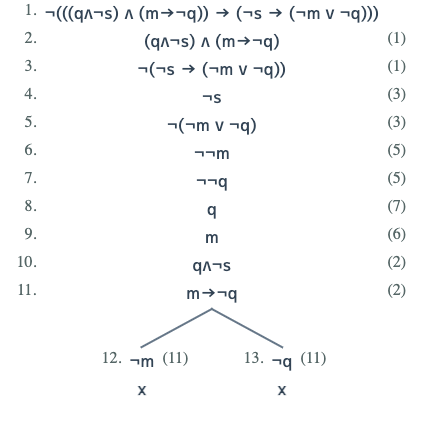
\includegraphics[width=0.5\linewidth]{C03//Images/logic-proof.png}
    \caption{A proof of the conclusion of the stack-exchange question}
    \label{fig:logic-proof}
\end{figure}
To read this proof, you need to know that $a \to b$ can be rewritten as $b \vee \neg a$, which I'll call the 'implication rule' for now. To prove the claim, the prover starts by assuming the implication is \textit{false}, and trying to derive from this some known-to-be-false statement(s). So line 1 assumes the negation of the desired conclusion. 

Applying the implication rule, and then negating $b \vee \neg a$ gives us $\neg v \wedge a$, and 'conjunction elimination' (saying that $A \wedge B$ tells you both $A$ and $B$) we get the assertions in lines 2 and 3. Doing the same thing to line 3 gives us the two facts in line 4 and 5. Applying negation to the $\vee$ in line 5, and then conjunction elimination, gets use the facts in lines 6 and 7. Double negation elimination gets us facts 8 and 9. 

Splitting fact 2 gets us facts 10 and 11. Applying the implication rule to fact 11, and then using conjunction-elimination, gets you $\neg q$ and $\neg m$, which contradict facts 8 and 9, hence we've derived a falsehood. 

The tool that provided that proof is a \emph{tableau solver} written by Wolfgang Schwarz of the University of Edinburgh. I include it here because you may be interested in the source code on github, and because "tableau solvers" are one of the many methods implemented by some of the tools in Isabelle. The  \href{https://en.wikipedia.org/wiki/Method_of_analytic_tableaux#:~:text=A%20tableau%20checks%20whether%20a,is%20unsatisfiable}{Wikipedia page} gives a nice summary of tableaux solvers. 

\section{More Interface Bits and Pieces}

While you were working through those proofs from Spivak, you probably got to the point where you said ``Hey\ldots was \isi{lt} defined in terms of \isi{gt} or the other way around? And was the rule for multiplication being commutative called ``\co{mul_commute}'', ``\co{mult_com'}', or one of 15 other possible variants? This is where the \co{sidekick} panel on the right comes in: it shows you everything in your theory. Want to jump to the definition of \isi{neg}? Click on it! By the way, if the Sidekick panel seems to not match what you've been typing, save your document, and the Sidekick contents will be refreshed. (Apparently updating while you're typing is problematic in some way, so updates are only triggered on save.)

Speaking of remembering/discovering things, if you open a proof document and (on a mac) press the command key (CTRL on Windows) while your cursor is above some term, you'll see something like this:



(I had command-hovered above the term ``A4complement'' to produce this.) Isabelle is telling me that this is a defined constant, namely a function from type a4Line to a4Line. This works in many panels of the interface, although I mostly use it in the main editor panel. 

On a closely-related note, sometimes you want to do the opposite thing: you want to do something to simplify an expression or prove a fact, and you know that the thing you need is (in the Spivak example) something to do with negation. But you cannot recall what small negation theorems you've already proved. You can, in a part of your proof document where you'd normally type a new theorem (right above the theorem you're currently working on is a good choice!) type \co{find_theorems neg}. Here, in a draft for a homework problem for this chapter that's based on the Spivak work you already did, is the result:

In the document itself:

In the output panel:
 

You'll notice that Isabelle has changed neg into ``neg'', and that's a general hint: the thing you're searching for may need parens. If at the same point I search for ``plus'', I get this:

where I've only shown the first two results. Isabelle has helpfully replaced ``plus'' with the special syntax we assigned to it; the extra parens around the symbol are there to make it into an infix operation (this is a messy detail that I'm not going to go into here). If you had tried typing \co{find_theorems} followed by the circled-plus-sign
you'd get an error message, because that symbol is just a bit too hard for Isabelle to deal with without it explicitly being identified as so-called 'inner syntax', i.e., the part of Isabelle that isn't ``theorem, using, by, fixes, assumes, shows, proof, have, show hence, qed''. But in fact if you type 
\begin{IS}
find_theorems 
\end{IS}
followed by the circled-plus in double-quotes,
you'd also get an error message, because Isabelle needs those extra parens to recognize that the circled-plus is the naming the infix addition function. 

Isabelle syntax oddities
I mentioned above that certain words --- things that show up in boldface in the interface --- are part of Isabelle's 'outer syntax', what you might think of as the syntax of Isabelle itself, while the stuff we write as facts are statements about mathematics, like ``a * b = b * a''. Those, in Isabelle, are called inner syntax. But Isabelle is very general, and defining new syntax is a possibility, so it's tough to give a complete description of either. The Isabelle Reference Manuals (available in the Documentation tab of the left-hand column of the interface) do so, but they're not easy to read! 

I think of various names that appear in Isabelle as somewhat liminal. I'm talking about names of theorems, for example, or of facts. If you're a traditional mathematician, you may be used to calling things ``theorem 1'' and ``theorem 2'', and so on. So go ahead and open up a proof document, and write a theorem called 1, and have it prove that 2 = 2. I recommend the fix-assume-show format. You could even write a proof for it by following the ``show'' part with ``by auto''  (This is the special shorthand proof where you don't even type the word ``proof'' or the closing ``qed''.) Isabelle will helpfully note that there are about 6 other ways that you could prove this as well. Now suppose for a moment that you decide that this is really the SECOND theorem in your document, but you've already labeled the next 6 theorems. You do what anyone might do: you decide to change its name to ``Theorem 1A''. Go ahead and try that. You'll get a (to me!) cryptic error message. But if you put the ``1A'' into double quotes, all is well. Those double-quotes don't really say ``I'm starting inner syntax here'', but rather ``this is something that's hard to parse unless I indicate the start and end of it''. It's the same thing that's happening with theory-document names: I have to call my document  \co{IbookCh1_exercises2} instead of  \co{IbookCh1-exercises2} because that hyphen makes it hard for Isabelle to parse it. If I wanted to use that name, the ``theory'' line at the head of my proof document would have to be 

theory "IbookCh1-exercises2"

with the double-quotes there to delimit the name for the sake of parsing. The same goes when you're naming facts during a proof. Numerical names like 0, 1, 2, are fine\ldots but ``1a'' needs quotes. And theorem 2.3? The ``2.3'' needs quotes. 

Quick summary: any time an apparently-innocuous change you make, typically involving punctuation or parsing something that could be number-like leads to a warning, maybe you need some double-quotes.

One more thing that you've probably already noticed: Isabelle is constantly re-parsing your proof document. That means that as you start to type a new lemma\ldots

the output panel is saying this:

You get a little farther: , and the output is 
You begin to indicate that it's lemma 3: , and the output is 
You keep typing, and at every character you type there are errors, until you've gotten to 
Where the error is 

When you finally finish typing 
shows "P=P"
only then are the errors all finally resolved. To be honest, I frequently copy-paste a previous theorem or lemma and then adjust the theorem name and what's fixed, assumed, or shown, one at a time, so that there's a little bit less of this (and so that I type less boilerplate). 

One more tip, although it's not actually an interface tip: you can put 
\begin{IS}
    declare [[show_types]]
\end{IS}
near the top of a proof document and thereafter the output panel will show things like this after the \isi{plus_assoc} theorem has been 'sorried':

If you want to show other things, you can extend the list, as in 
\begin{IS}
declare[[show_types, show_abbrevs, sh ...]]
\end{IS}
and as you type that last ``sh'' a list of other things you might want to show is offered as a tool-tip. I seldom use these, but \co{show_types} may be useful to you as you're getting started. 

Getting to proofs faster and more simply
One thing you might have learned from the Spivak proofs is that most of the time, you knew something (fact1) and you had something else (fact2) that relates this to some other thing, and you applied fact2 to fact1 to get some new ``fact1'' for the next step. There's seldom a 'big picture' situation where you needed to combine 7 things all at once to get an answer. On the other hand, if you resorted to sledgehammer, you found that it sometimes did exactly this combination of 14 different items to do a whole lot of steps privately and then just say ``yep\ldots I got it!'' You might be wishing you could do the same thing. But if you look at the proof state during the middle of a proof, there's typically just one fact in your bag of facts (``this''), and you have to pull in fact2 be realizing that some theorem could be applied to ``this'', or some definition would let %you transform ``this'', etc. In the meantime, ``by auto'' seems to be doing a lot of things under the hood: if %a simple deduction leads to \co{(Z \negequal Z) \/ x \in P}, for instance, ``auto'' may be able to conclude %that x is in P, because the first clause of the ``or'' is false, so the second must be true. How's it doing %that? 

% XXX Fix broken text above

Broadly speaking, many proofs in Isabelle amount to glorified simplification. That simplification might be as simple as replacing \co{False \/ Q} with just Q, or might be more complex, like replacing all occurrences of the ``difference'' function with their definition, i.e., diff a b ≡ (a ⊕ (neg b)). It might amount to replacing \co{cos^2(t) + sin^2(t)} with 1, where t could be some arbitrarily complicated expression. In all cases, one of the key points about simplification is that it should reduce some well-defined measure of complexity, i.e., always go downhill. You definitely don't want one of your simplification rules to be a + b = b + a, because that can be applied infinitely often without making any progress. 

Isabelle has a simplifier, and it's freaking amazing. It's at the heart of auto; it's what ``simp'' uses; it's part of lots of provers. It uses a set of simplification rules, often described as the ``simp set'' or ``simpset'', and you, the user, can add to that set of rules during a proving session. Adding a rule like ``a + b = b + a'' is a bad idea obviously, but saying ``let's always get rid of all occurrences of 'diff''' actually sounds pretty good. To add a theorem to the simpset, you put [simp] just before the colon, as in 


Now whenever you need to change ``a + Z'' to just ``a'', you no longer need to say \isi{using additive_ident}, because it's in the simpset, and if you're doing a proof by auto or simp, it'll be seen. (There may be other provers that don't necessarily refer to the simpset, but this already takes you a long way.)

In much the same way, there are ``introduction'' and ``elimination'' rules beyond those mentioned in natural deduction, and you can add to the introset and elimset in the same way. The rule that says to replace every occurrence of \isi{diff a b} with \isi{a + neg b} might be considered both an elimination rule and a simplification rule, so you could put ``[simp, elim]'' before the colon. Good Isabelle users add simplification, introduction, and elimination rules whenever possible, within limits. Imagine that you've defined the Fibonacci numbers recursively. Eliminating \isi{fib} in \isi{fib 4} might produce \isi{ (fib 3_ + (fib 2)}, which elimination then changes to \isi{fib 2 + fib 1 + fib 1 + fib 1}, and then \isi{fib 1 + fib 1 + fib 1 + fib 1 + fib 1}, which finally can be converted to \isi{1 + 1 + 1 + 1+ 1}. That's OK in this simple example, but what if it had been \isi{fib 20}? You really don't want to produce $2^20$ terms, right? 

Why would you want an introduction rule, though? Why not just get rid of all occurrences of diff during your proof? Well, what if the goal is to show that ``diff a b \in P''? You either need to eliminate the ``diff'' from the goal somehow (and we haven't really considered that yet), or you need a way to introduce a diff in the last step of your proving, so that you have something that unifies with the goal. 

To see what adding ``simp'' can do for a proof, let's take a look back at the Spivak exercises from Chapter 1. One of them was this, where I've written out a complete solution, taking seven steps to do it. This is great as a mirroring of Spivak's proof, but that's not really Isabelle's goal -- it's not a pedagogical tool so much as a proof-verifier, so a simple ``yup, here's a brief proof in a form you can't really understand, but which I can prove is correct'' line in a proof document is considered a Good Thing. Let's see whether we can get to that for exercise 3. 
\begin{IS}
    
lemma ex3: 
  fixes x::r and a and b
  assumes "x ⊕ a = b"
  shows "x = b ⊖ a"

proof -
  have 0: "x ⊕ a = b" using assms by auto
  have 1: "(x ⊕ a) ⊕ (neg a) = b ⊕ (neg a)" using 0 by auto
  have 2: "(x ⊕ a) ⊕ (neg a) = x ⊕ (a ⊕ (neg a))" using plus_assoc by auto
  have 3: "x ⊕ (a ⊕ (neg a)) = b ⊕ (neg a)" using 1 2 by auto
  have 4: "x ⊕ Z = b ⊕ (neg a)" using 3 negation(1) by auto
  have 5: "x = b ⊕ (neg a)" using 4 additive_ident(1) by auto
  show ?thesis using 5 diff_def by auto
qed
\end{IS}

As a first step, we can replace \isi{have n: ... using n-1 ...} by using \isi{hence}, and do the same for the final \isi{show} by changing it to \isi{then show}:
\begin{IS}
    
proof -
  have 0: "x ⊕ a = b" using assms by auto
  hence 1: "(x ⊕ a) ⊕ (neg a) = b ⊕ (neg a)" by auto
  have 2: "(x ⊕ a) ⊕ (neg a) = x ⊕ (a ⊕ (neg a))" using plus_assoc by auto
  have 3: "x ⊕ (a ⊕ (neg a)) = b ⊕ (neg a)" using 1 2 by auto
  hence 4: "x ⊕ Z = b ⊕ (neg a)" using negation(1) by auto
  hence 5: "x = b ⊕ (neg a)" using additive_ident(1) by auto
  then show ?thesis using diff_def by auto
qed
\end{IS}

At this point, 0, 3, 4, and 5 can be eliminated because they're never used. In going from 3 to 4, we use the fact that a + (neg a) is Z (i.e., zero), which appears a few lines before as 
\begin{IS}
lemma  negation: (* Spivak calls this P3 *)
  fixes a::r
  shows "a ⊕ (neg a) =  Z"
  and  "(neg a) ⊕ a =  Z"
  sorry
\end{IS}

Let's add the [simp] attribute to this theorem:

\begin{IS}
lemma  negation [simp]: (* Spivak calls this P3 *)
...
\end{IS}
Now we can change things to read
\begin{IS}
have 3: "x ⊕ (a ⊕ (neg a)) = b ⊕ (neg a)" using 1 2 by auto
hence 4: "x ⊕ Z = b ⊕ (neg a)" by auto
\end{IS}

But if auto can do both those steps, can it do them both at the same time? Yes! We can change things to 
\begin{IS}
  have 0: "x ⊕ a = b" using assms by auto
  hence 1: "(x ⊕ a) ⊕ (neg a) = b ⊕ (neg a)" by auto
  have 2: "(x ⊕ a) ⊕ (neg a) = x ⊕ (a ⊕ (neg a))" using plus_assoc by auto
  hence 4: "x ⊕ Z = b ⊕ (neg a)" using 1 2  by auto
  hence 5: "x = b ⊕ (neg a)" using additive_ident(1) by auto
  then show ?thesis using diff_def by auto
\end{IS}

Now converting \isi{x + Z} to just \isi{x} is another pretty obvious simplification, so we can go back to the \isi{additive_ident} theorem and add \isi{[simp]} there as well/

And now line 5 becomes
\begin{IS}    
hence 5: "x = b ⊕ (neg a)" by auto
\end{IS} 
And once again, this can be combined with the use of auto in line 4, so that we have
\begin{IS}
proof -
  have 0: "x ⊕ a = b" using assms by auto
  hence 1: "(x ⊕ a) ⊕ (neg a) = b ⊕ (neg a)" by auto
  have 2: "(x ⊕ a) ⊕ (neg a) = x ⊕ (a ⊕ (neg a))" using plus_assoc by auto
  hence "x = b ⊕ (neg a)" using 1 2 by auto
  then show ?thesis using diff_def by auto
qed
\end{IS} 
where I've eliminated label "5" because it was no longer in use. At this point, going from fact 0 all the way to fact formerly-5 involves just repeated applications of auto, except that we've used the assumption (at fact 0) and \isi{plus_assoc} (at fact 2). Let's try a big step and combine them all!

Wow! That proof sure is getting shorter! If we look at the proof state with the cursor at the end of the ``have" line, it says that we know x = b + (neg a), and we want to show that x = b - a. Well, those are connected by the definition of ``diff'', as suggested in the ``show'' line. So we could, in fact, turn this into one line:

\begin{IS}    
show ?thesis using  assms plus_assoc  diff_def by auto
\end{IS} 

\ldots but let's hold off on that for a moment. Rather that using \isi{diff_def} to push things further towards the goal, we're going to use it to simplify the goal:

If you place the cursor in the location shown, you can see that the goal has been modified. Try putting the cursor both before and after the \isi{unfolding diff_def} so see the change. After the unfolding, the goal becomes 

\ldots which is what we've already managed to reach. So we can write a final idiomatic proof:

In summary: adding a few things to the simpset made our proof a lot shorter and simpler. Using ``unfolding'' let us simplify the goal a little. But as a result of doing all these steps, the didactic message of Spivak's presentation was lost. 


What's the simplifier doing???
Why does it break the proof of the next lemma when we add ``negation'' to the simp-set? 

Time to talk about what various provers are doing: auto does a lot of simplification (using what rules? WE get to tell it!) Blast is similar, but doesn't know about equality. 

And now we can say what ``using'' is doing: it's saying to the prover ``here's a fact you might find useful''\ldots which the prover may ignore. By contrast, there's a similar thing, 'unfolding': this replaces function applications with their definitions (or more generally, the left side of an equality with the right side). 

\subsection{The triangle inequality}
Having worked through a few pages of Spivak in detail, I really wanted to finish the triangle inequality proof. Spivak's own proof turned out to be messy for me to write, so I came up with my own. It was based on a few key lemmas: 
\begin{enumerate}
    \item For $x$ nonnegative, we have $|x| = x$.
    \item For $x$ negative, we have $|x| = -x$.
    \item For all $x$, we have $x \le |x|$.
    \item For all $x$, we have $|x| = |-x|$
\end{enumerate}
Now if $x+y$ is nonnegative, we have
$$
|x+y| = x + y
$$
by the first rule, and each of $x$ and $y$ is no larger than its absolute value, so we have $$
x + y \le |x| + |y|,$$
and we're done with this case. Hidden in there was the transitivity of less-than-or-equal, and the fact that if $a \le b$ and $c \le d$ then $a + c \le b + d$, small lemmas I had to prove along the way. 

What if $x + y$ is negative? Then we can apply the first case to $-(x+y) = -x + -y$, to conclude that 
$$
|-(x+y)| \le |-x| + |-y|.$$

The left hand side is the same as $|x+y|$ by the fourth lemma. The right hand side is the same as $|x| + |y|$, by the fourth lemma, applied twice. And that concludes the proof. 

In a math text, I might have written "To prove the triangle inequality, it suffices to prove it when $x + y$ is nonnegative, because if it's negative..." and then followed with the previous two paragraphs. In Isabelle, I can mimic the same thing using the keyword \isi{presume}. The theorem might look like this:
\begin{IS}
theorem triangle_inequality:
  fixes x y
  shows "abs(x + y) le abs(x) + abs(y)"
\end{IS}
where \isi{abs} has already been defined as the absolute value function, and \isi{le} has been defined as less-than-or-equal. Let's also suppose that \isi{ge} has been defined as greater-than-or-equal, and \isi{Z} is, as before, or symbol for zero. The proof might continue
\begin{IS}
theorem triangle_inequality [known]:
  fixes x y
  shows "(abs (x ⊕ yb)) le  ((abs x)  ⊕ (abs y))"
proof -
  presume A: "⟦x gt Z; y gt Z⟧ ⟹ (abs (x ⊕ y)) le  ((abs x)  ⊕ (abs y))"
  show ?thesis  
  proof -
    \textit{lots of steps here, some using the presumed fact A}
  qed 
next
  show "⟦x gt Z; y gt Z⟧ ⟹ (abs (x ⊕ y)) le  ((abs x)  ⊕ (abs y))"
  proof -
     \textit{lots of steps here too}
  qed
qed
\end{IS}

The "presumes" part is just another way of writing the fixes-assumes-shows statement of a theorem that we've already seen --- between the double brackets are the 'assumes' parts separated by semicolons; the long double arrow means "shows", and the conclusion is on the right. Once we've presumed something
we can use it in a proof. When we're done concluding the main claim, we still need to go back and prove the bit that "it suffices to show" --- that's the part following the \isi{next}. Unfortunately, the name \isi{?thesis} doesn't get bound to this, so we have to explicitly re-state the presumed fact. 

This conversion of our "it suffices to show" proof into Isabelle is a little awkward, and if we'd said in some proof "to prove C, it suffices to prove A and B, because ...", i.e., if we'd had \textit{two} presumptions, then things are even messier. My personal (regretful) conclusion is that it's best to separate the presumed fact out into a lemma, and then apply it in the proof of the main theorem. 

\subsection{Fact sets, proof structures}
In the course of doing the triangle inequality proof, I found a \textit{ton} of little lemmas that I needed, like "if x is greater than y, then x is \textit{not} less-than-or-equal-to y", and "if x is greater than y, then x is greater-than-or-equal-to y". When you introduce something like "less than", it's worth proving as many tiny facts about it as possible, so that its definition is almost beside the point. 

One consequence of this is that I ended up using the sidekick a lot --- it's a quick table of theorems that you can click on to jump to a definition. (Once you jump there, you can use the arrow buttons on the menu bar to jump back to where you were just working!) Even with this help, things felt slow. So I did an experiment. 

What if, as I was trying to prove a lemma, all the prior lemmas were in the collection of known facts for me to use? Just as you can add a lemma to the simpset that the simplifier uses, you can create your own fact set and add things to it. I typed \isi{named_theorems known} to create a new set of facts with the not-very-inventive name `known'. Note: \isi{named_theorems} is another Isabelle/Isar keyword. 

Then each time I wrote a lemma, I'd include `known' like this: \isi{lemma le_gt [known]:}, which would add the lemma \isi{le_gt} to my fact-set once it was proved. 

Unfortunately, I didn't find an easy way to do something this simple with definitions, so after a definition, I'd have to write
\begin{IS}
definition le::"r ⇒ r ⇒ bool"
  where "le a b = ge b a" 

declare le_def[known]
\end{IS}
Here the keyword \isi{declare} is used to say that you want to add \isi{le_def} (the "fact" that \isi{le} is defined as shown above, automatically created whenever anything is defined) to the fact-set \isi{known}. 

(It turns out that there \textit{is} a way to add an attribute to a definition, and it looks like this:
\begin{IS}
definition le::"r ⇒ r ⇒ bool"
  where [known]: "le a b = ge b a" 
\end{IS}
which I find less satisfactory, because of the requirement of that extra colon -- it feels inconsistent with the syntax for attributes elsewhere. But clearly both are OK.)

With this done, most of the proofs became simply something like
\begin{IS}
proof -
  show ?thesis using known assms by auto
qed
\end{IS}
No more 12-line proofs! Far fewer case-based proofs! It's wonderful! 

To be fair, I should say that it's not \textit{completely} wonderful. Sometimes the \isi{by auto} had to be \isi{by metis}, or \isi{by meson}, and I had to find those things using \isi{try} or \isi{sledgehammer}. And the resulting proof gives no clue to the reader about what facts were actually needed, and what others were just along for the ride. Finally, there's clearly a limit to this approach --- what happens when your fact set has 10,000 items in it? Well, that's the situation that sledgehammer lives with: it's got everything proved so far in any included theory, and every named theorem from the current theory, in its toolbox. It takes a while to come up with proofs, too. Finally, the proof-state display gets so cluttered that it's almost impossible to read, which is bad when you reach a situation where you have to nudge things along by hand. 

In short: it was an interesting experiment, but it's not the way to work in general. 

\section{Beginner tips}
When you start proving things in Isabelle, challenges abound. You get partway through a proof, and find that sledgehammer cannot complete it. You're trying to do an incredibly simple proof and "auto" can't seem to help. You look in the proof state and see that "this" is exactly your goal, but can't close out the proof. You see that you want to prove \isi{a ===> b}, and you've already established \isi{b}. Why isn't the overall goal obvious? 

I cannot answer all these questions for you, because some depend on context, but I can give some hints. 

\begin{itemize}
    \item Watch for errors! If there's a red marker beside a line where you're trying to do a proof, move your cursor into that line and see what error appears in the output window. Fix it before trying to prove anything!

    \item Use quotation marks! Sometimes a fact-name or an imported-theory-name needs them. But sometimes it's more subtle. Consider the following small theorem:
\begin{IS}    
theorem join_containsL:
  fixes P Q
  assumes "P ≠ Q"
  shows "P ≠ Q"
proof -
  show P ≠ Q using assms try 
...
\end{IS}
The first mistake here is that you probably want to use the more idiomatic \isi{show ?thesis} as a matter of habit, but perhaps you're still learning and want to write out explicitly the thing you're trying to show. It seems totally obvious, but neither 'try' nor 'sledgehammer' can get anywhere. What's wrong? You need to put \isi{P \\<notequal> Q} in quotes:
\isi{show "P \\<notequal> Q" using assms by auto} works fine. 

\item Use Isabelle's color-coding hints! Here's a lemma I proved about "A2", the 2-dimensional affine plane:
\begin{figure}[h]
    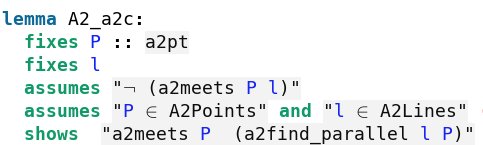
\includegraphics[width=0.5\linewidth]{C03/Images/good-statement.png}
\end{figure}

Contrast that with this incorrect lemma statement:
\begin{figure}[h]
    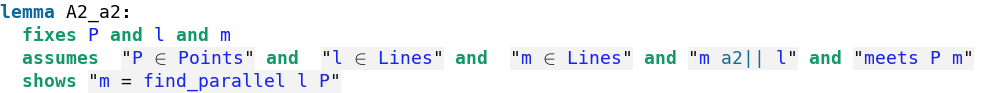
\includegraphics[width=\linewidth]{C03/Images/bad-statement.png}
\end{figure}
They really look pretty similar, but in the second lemma, I've used "Points" and "Lines" rather than "A2Points" and "A2Lines". The first two have not been defined, while the second two have. That makes the first two "free" variables -- it's as if my theorem statement said "For all sets Points and Lines, if P is in Points and ..."
That's not what I intended at all. The big clue here is the color: in the first theorem statement, \isi{A2Points} is in black, indicating a bound variable. In the second, \isi{Points} is in blue, indicating a free variable (one that will be implicitly included in a 'forall' at the start of the lemma. (The same goes for \isi{meets} and \isi{find_parallel}.) Informal summary: "Red is horrible. Blue is probably bad." 

\item Check to be sure that you're trying to prove what you're trying to prove. By this I mean "check that the 'shows' part of 'fixes-assumes-shows' actually states the thing you were hoping to prove, rather than something close to it." Copy-paste can make a fool of you here. Free variables, as in the last example, can be a problem. Simple typos can be a problem. One general clue is that if you're trying to prove something that seems easy, but \isi{sledgehammer} can't do it, there's a good chance it's not actually true. Check that all the necessary assumptions are there; check that the desired conclusions express the right thing. Check that the names are all correct. Only after all that should you start to dig deeper. 

\end{itemize}